\documentclass[sigconf,nonacm]{acmart}

\usepackage{booktabs}
\usepackage{amsmath}
\usepackage{amsfonts}
\usepackage{algorithm}
\usepackage{algorithmic}
\usepackage{graphicx}
\usepackage{makecell}
\usepackage{microtype}
\usepackage{balance}

\makeatletter
\newcommand\captionof[2]{\def\@captype{#1}\caption{#2}}
\makeatother

\settopmatter{printacmref=false}

% Conference metadata






\pagestyle{plain}
\begin{document}

\title{Adaptive Quantum-Resistant Hybrid Cloud Storage With Zero-Trust Key Distribution}

\author{Madhira Venkata Ramesh Reddy}
\affiliation{%
  \institution{SRM University-AP}
  \department{Department of Computer Science and Engineering}
  \city{Neerukonda, Amaravati}
  \state{Andhra Pradesh}
  \country{India}
}
\email{ramesh_madhira@srmap.edu.in}

\author{Varsha Sambhaje}
\authornote{Corresponding author: Varsha Sambhaje, email: varsha.s@srmap.edu.in}
\affiliation{%
  \institution{SRM University-AP}
  \department{Quantum Technology \& Institute}
  \department{Department of Computer Science and Engineering}
  \streetaddress{Neerukonda}
  \city{Amaravati}
  \state{Andhra Pradesh}
  \postcode{522240}
  \country{India}
}
\email{varsha.s@srmap.edu.in}

\renewcommand{\shortauthors}{}

\begin{abstract}
Quantum computers running Shor's algorithm threaten cloud storage by breaking RSA/ECC public-key cryptography, enabling Harvest Now, Decrypt Later (HNDL) attacks. Direct deployment of post-quantum primitives like NIST ML-KEM (CRYSTALS-Kyber) introduces key expansion ($12.5\times$), WAN fragmentation, and centralized key exposure. We design, formally verify, and evaluate a multi-layered quantum-resistant hybrid cloud storage architecture synthesizing five defenses: (1)~an Adaptive Encryption Decision Engine (AEDE) matching cipher strength to payload sensitivity and size; (2)~a Dual-Key Hybrid KEM combining SECP256R1 and Kyber-512 via HKDF-SHA256 ensuring classical-quantum IND-CCA2 security; (3)~Zero-Trust Shamir (2,3)-threshold sharing over GF(257) eliminating single-point repository exposure; (4)~an Early-Drop outer HMAC-SHA256 boundary filter dropping forged requests in 0.089~ms ($12.3\times$ speedup against DoS); and (5)~an append-only SHA-256 hash-chain audit ledger. Symbolic verification in ProVerif 2.05 proves master key secrecy. Xeon benchmarks show hybrid encryption incurs only 1.28~ms overhead for 1~MB payloads (0.16~ms delta over ECC), with 79\% AVX-512 energy reduction.
\end{abstract}

\begin{CCSXML}
<ccs2012>
   <concept>
       <concept_id>10002978.10002979.10002981</concept_id>
       <concept_desc>Security and privacy~Public key (asymmetric) techniques</concept_desc>
       <concept_significance>500</concept_significance>
   </concept>
   <concept>
       <concept_id>10002978.10002979.10002984</concept_id>
       <concept_desc>Security and privacy~Key management</concept_desc>
       <concept_significance>500</concept_significance>
   </concept>
   <concept>
       <concept_id>10002978.10003014.10003015</concept_id>
       <concept_desc>Security and privacy~Distributed systems security</concept_desc>
       <concept_significance>500</concept_significance>
   </concept>
   <concept>
       <concept_id>10002978.10003014.10003017</concept_id>
       <concept_desc>Security and privacy~Denial-of-service attacks</concept_desc>
       <concept_significance>300</concept_significance>
   </concept>
</ccs2012>
\end{CCSXML}

\ccsdesc[500]{Security and privacy~Public key (asymmetric) techniques}
\ccsdesc[500]{Security and privacy~Key management}
\ccsdesc[500]{Security and privacy~Distributed systems security}
\ccsdesc[300]{Security and privacy~Denial-of-service attacks}

\keywords{Post-Quantum Cryptography, NIST ML-KEM, CRYSTALS-Kyber, Hybrid KEM, Shamir Secret Sharing, GF(257), Zero-Trust Architecture, Denial-of-Service Mitigation, Cloud Storage Security, Harvest Now Decrypt Later}

\maketitle
\pagestyle{plain}
\fancyhead{}


% Declared right after maketitle to float to the top of Page 2
\begin{figure*}[t]
\centering
\includegraphics[width=0.96\textwidth]{fig1_wide.png}
\caption{End-to-end architecture of Quantum-Resistant Adaptive Hybrid Cloud Storage, illustrating multi-tenant client profiling, dual-key encapsulation, early-drop HMAC validation, and zero-trust Shamir secret sharing across isolated storage domains.}
\label{fig:arch}
\end{figure*}

\section{Introduction}
Enterprise cloud storage relies on public-key ciphers (RSA-3072, Elliptic Curve Cryptography (ECC-256))~\cite{boneh2020graduate} secured by the Integer Factorization Problem (IFP) and the Elliptic Curve Discrete Logarithm Problem (ECDLP)~\cite{katz2020introduction}. While classical algorithms require sub-exponential $\mathcal{O}(\exp((c + o(1))(\ln n)^{1/3}(\ln \ln n)^{2/3}))$ or exponential $\mathcal{O}(\sqrt{p})$ time, Shor's algorithm~\cite{shor1994algorithms} breaks both in polynomial time $\mathcal{O}(n^3)$. A $\sim$4,000-qubit quantum device compromises RSA/ECC in seconds, empowering adversaries to execute HNDL attacks on 50-year regulatory archives such as HIPAA and financial records~\cite{mosca2022quantum}. Naive deployment of NIST ML-KEM (CRYSTALS-Kyber)~\cite{bos2018crystals,avanzi2021crystals} \mbox{introduces} three critical operational barriers:\nopagebreak
\begin{enumerate}
    \item \textbf{Key Expansion Overhead:} Kyber-512 public keys require 800 bytes, representing a $12.5\times$ expansion over SECP256R1 (65 bytes).
    \item \textbf{WAN MTU Fragmentation:} Combined lattice public keys and ciphertexts exceed standard 1500-byte Wide Area Network (WAN) Maximum Transmission Unit (MTU) boundaries, resulting in packet fragmentation and connection latency penalties.
    \item \textbf{Central Repository Exposure:} Centralized Key Management Services (KMS) present single-point targets for catastrophic database exfiltration~\cite{sahai2021use}.
\end{enumerate}

\noindent\textbf{Contributions.} We deliver five core technical contributions:
\begin{itemize}
    \item A holistic multi-layered quantum-resistant cloud storage architecture harmonizing dynamic client profiling with server-side zero-trust repositories.
    \item An IND-CCA2 dual-key hybrid Key Encapsulation Mechanism (KEM) combining SECP256R1 Elliptic Curve Diffie-Hellman (ECDH) and Kyber-512 via HKDF-SHA256, guaranteeing security against both classical and quantum adversaries.
    \item Zero-Trust Shamir secret sharing over the Galois Field GF(257) ensuring zero Shannon mutual information for any single repository breach.
    \item An Early-Drop outer HMAC-SHA256 boundary filter rejecting forged payloads in 0.089~ms, achieving a $12.3\times$ speedup against CPU-exhaustion Denial-of-Service (DoS) floods.
    \item Formal verification in ProVerif 2.05 confirming master key secrecy and boundary invariance, backed by bare-metal Xeon microbenchmarks across 100~KB--10~MB payloads.
\end{itemize}

\section{Related Work and Architectural Comparison}
Post-Quantum Cryptography (PQC) transition efforts have predominantly focused on hybrid KEM theoretical formulations~\cite{bindel2019hybrid,eller2021new,stebila2023hybrid,stebila2016post}. In storage environments, classical Shamir secret sharing~\cite{shamir1979share} has been applied for fault tolerance, but has not been integrated with lattice encapsulation, early-drop DoS defenses, and tamper-evident audit chains. Table~\ref{tab:comparison} contrasts existing security models with our proposed adaptive hybrid architecture.

\begin{table}[t]
\centering
\caption{Architectural comparison of security paradigms.}
\label{tab:comparison}
\scriptsize
\setlength{\tabcolsep}{1.2pt}
\begin{tabular}{lcccccc}
\toprule
\textbf{Scheme} & \textbf{PQC} & \textbf{Fallback} & \textbf{Split} & \textbf{Telemetry} & \textbf{DoS} & \textbf{Ledger} \\
\midrule
Pure ECC & No & Yes & No & No & No & Opt. \\
Pure Kyber & Yes & No & No & No & No & Opt. \\
Hybrid TLS 1.3 & Yes & Yes & No & Partial & No & No \\
KMS Cluster & Opt. & Opt. & Yes & No & No & Yes \\
\textbf{Proposed} & \textbf{Yes} & \textbf{Yes} & \textbf{2-of-3} & \textbf{AEDE} & \textbf{0.089 ms} & \textbf{SHA-256} \\
\bottomrule
\end{tabular}
\end{table}

\section{System Architecture and Methodology}
The architecture synchronizes three primary functional layers with tamper-evident auditing (Fig.~\ref{fig:arch}): (1)~\emph{Client Ingestion \& Profiling}; (2)~\emph{Gateway Routing \& Early-Drop DoS Filter}; and (3)~\emph{Zero-Trust Key Splitting \& Distributed Repositories}.

\subsection{Adaptive Encryption Decision Engine (AEDE)}
AEDE dynamically selects the optimal cryptographic pipeline based on payload sensitivity $S \in [0, 1]$ and file size $F$ (in bytes):
\begin{equation}
\label{eq:profile}
\mathit{Profile}(S, F) = 
\begin{cases}
\text{Hybrid-GCM}, & \text{if } S \ge 0.7 \lor (S \ge 0.4 \land F < 10\text{ MB}), \\
\text{Kyber-GCM}, & \text{if } S \ge 0.4 \land F \ge 10\text{ MB}, \\
\text{ECC-GCM}, & \text{otherwise}.
\end{cases}
\end{equation}
This policy eliminates unnecessary quantum overhead for transient or low-sensitivity data while enforcing full hybrid defense for mission-critical archives.

\subsection{Dual-Key Hybrid KEM}
To guarantee forward secrecy against future quantum attacks without sacrificing classical compliance, the client generates dual shared secrets: classical $S_{ecc}$ via SECP256R1 ECDH and post-quantum $S_{kyber}$ via Kyber-512 KEM. The master session key $K_{master}$ is derived using the HMAC-based Key Derivation Function (HKDF-SHA256):
\begin{align}
K_{hybrid} &= \text{HKDF-Extract}(salt, S_{ecc} \parallel S_{kyber}), \label{eq:khybrid} \\
K_{master} &= \text{HKDF-Expand}(K_{hybrid}, info, 32). \nonumber
\end{align}
By the dual-PRF property of HKDF~\cite{krawczyk2010hmac}, $K_{master}$ remains indistinguishable from random unless an adversary solves both ECDLP and Module Learning With Errors (Module-LWE) simultaneously.

\subsection{Zero-Trust Key Distribution via Shamir Sharing over GF(257)}
Rather than storing $K_{master}$ in a centralized key vault, the gateway splits the 32-byte secret into three shares using a (2,3)-threshold Shamir secret sharing scheme over the finite field $GF(257)$. For each byte $b \in [0, 255]$:
\begin{equation}
\label{eq:shamir}
f_b(x) = (b + a_1 x) \bmod 257, \quad a_1 \in_R [0, 256].
\end{equation}
The secret is reconstructed via Lagrange interpolation using any two distinct shares:
\begin{equation}
\label{eq:lagrange}
b = f(0) = \sum_{j \in \{1,2\}} y_j \prod_{m \ne j} (-x_m)(x_j - x_m)^{-1} \bmod 257.
\end{equation}
$Share_1$ is encapsulated in the object metadata header, $Share_2$ is committed to an encrypted PostgreSQL database, and $Share_3$ is escrowed in an offline air-gapped Hardware Security Module (HSM). Compromising any single repository yields zero Shannon mutual information: $I(K_{master}; Share_i) = 0$.

\subsection{Early-Drop Outer HMAC Boundary Verification}
Post-quantum decapsulation requires significant CPU compute ($1.095$~ms in unoptimized pipelines). Attackers could forge invalid ciphertexts to cause CPU saturation. To neutralize this vector, the client signs fixed-length container headers using an outer Hash-based Message Authentication Code (HMAC-SHA256) key $K_{gw}$ pre-shared during tenant onboarding (Table~\ref{tab:layout}, Algorithm~\ref{alg:lifecycle}).

\begin{table}[t]
\centering
\caption{Structured container layout and cryptographic roles.}
\label{tab:layout}
\scriptsize
\setlength{\tabcolsep}{1.5pt}
\begin{tabular}{p{2.3cm} p{1.6cm} c p{3.2cm}}
\toprule
\textbf{Segment} & \textbf{Component} & \textbf{Size} & \textbf{Cryptographic Function} \\
\midrule
Protocol Header & Magic+Ver+Suite & 6 B & Format validation ('QSTO', v02) \\
Payload Nonce & Deterministic IV & 12 B & Nonce for Advanced Encryption Standard Galois/Counter Mode (AES-256-GCM) \\
Zero-Trust Share & Shamir Share 1 & 32 B & $x=1$ share over GF(257) \\
Hybrid KEM Data & ECC pk + Kyber ct & 833 B & Dual-key exchange material \\
Boundary Envelope & Outer HMAC-SHA256 & 32 B & 0.089 ms Early-Drop filter \\
Encrypted Body & Tag + Ciphertext & 16B+ & Encrypted object payload \\
\bottomrule
\end{tabular}
\end{table}

\begin{algorithm}[t]
\caption{Adaptive Ingestion, Early-Drop, and Reconstruction}
\label{alg:lifecycle}
\scriptsize
\begin{algorithmic}[1]
\REQUIRE Payload $P$, sensitivity $S$, tenant $T$, gateway key $K_{gw}$.
\ENSURE Encrypted container $\Omega$, or error $\bot$.
\STATE $Mode \leftarrow \text{AEDE\_Profile}(S, |P|)$; $K_{master} \in_R \{0, 1\}^{256}$; $IV \in_R \{0, 1\}^{96}$
\STATE $C, Tag_{gcm} \leftarrow \text{AES256-GCM-Encrypt}(K_{master}, IV, P, AAD)$
\STATE $(Share_1, Share_2, Share_3) \leftarrow \text{Shamir\_Split}(K_{master}, 2, 3)$
\STATE $(pk_{ecc}, sk_{ecc}) \leftarrow \text{KeyGen}_{\text{ECC}}()$; $(C_{ecc}, S_{ecc}) \leftarrow \text{Encaps}_{\text{ECC}}(pk_{gw,ecc})$
\STATE $(C_{kyber}, S_{kyber}) \leftarrow \text{Kyber\_Encaps}(pk_{gw,kyber})$
\STATE $Header \leftarrow Magic \parallel Version \parallel Mode \parallel IV \parallel Share_1 \parallel pk_{ecc} \parallel C_{kyber}$
\STATE $Tag_{hmac} \leftarrow \text{HMAC}(K_{gw}, Header)$
\STATE Store $Share_2$ in DB; Emit audit hash $H_k$; $\Omega \leftarrow Header \parallel Tag_{hmac} \parallel Tag_{gcm} \parallel C$; \textbf{return} $\Omega$
\STATE \textbf{Early-Drop Check at Socket Boundary:}
\STATE \textbf{if} $|\Omega| < 931$ B $\lor$ $\Omega[0:4] \neq \texttt{'QSTO'}$ \textbf{then return} $\bot_{fmt}$
\STATE \textbf{if} $\text{HMAC}(K_{gw}, \Omega[0:909]) \neq \Omega[909:941]$ \textbf{then return} $\bot_{hmac}$
\STATE $S_{ecc} \leftarrow \text{Decaps}_{\text{ECC}}(sk_{gw}, C_{ecc})$; $S_{kyber} \leftarrow \text{Kyber\_Decaps}(sk_{gw}, C_{kyber})$
\STATE Fetch $Share_2$ from DB; $K_{master} \leftarrow \text{Shamir\_Reconstruct}(\{Share_1, Share_2\})$
\STATE $P \leftarrow \text{AES256-GCM-Decrypt}(K_{master}, IV, C, Tag_{gcm})$; \textbf{return} $P$
\end{algorithmic}
\end{algorithm}

\subsection{Forensic Hash-Chain Audit Ledger}
All storage lifecycle transactions are appended to an immutable, cryptographically linked hash chain:
\begin{equation}
\label{eq:hashchain}
H_k = \text{SHA256}(H_{k-1} \parallel E_k \parallel T_k \parallel \mathit{ID}_k),
\end{equation}
where $E_k$, $T_k$, and $\mathit{ID}_k$ represent event data, timestamp, and tenant identity. Tampering with any historical audit entry invalidates all subsequent hashes, providing instantaneous mathematical evidence of tampering. Automated anomaly detection evaluates rolling log-likelihood under a trained Dirichlet distribution.

\section{Formal Security and Threat Analysis}

\begin{theorem}[IND-CCA2 Security \& Quantum Forward Secrecy]
Let $\Pi_{hybrid}$ be the dual KEM combining SECP256R1 and Kyber-512 via HKDF-SHA256. If either SECP256R1 is CDH-secure or Kyber-512 is IND-CCA2 secure under Module-LWE, then $\Pi_{hybrid}$ is IND-CCA2 secure against quantum adversaries.
\end{theorem}
\begin{proof}
An adversary $\mathcal{A}$ breaking $K_{hybrid}$ implies breaking the HKDF extraction lemma. Since $K_{hybrid} = \text{HKDF}(S_{ecc} \parallel S_{kyber})$, the derived key is computationally indistinguishable from uniform unless $\mathcal{A}$ solves both ECDLP and Module-LWE. Shor's algorithm solves ECDLP in polynomial time but cannot solve lattice-based Module-LWE. Hence, quantum forward secrecy holds unconditionally against classical-quantum hybrid adversaries.
\end{proof}

\begin{theorem}[Information-Theoretic Key Confidentiality]
Let $K_{master}$ be split via Shamir (2,3) sharing over GF(257). An adversary accessing fewer than 2 shares possesses zero Shannon mutual information regarding $K_{master}$.
\end{theorem}
\begin{proof}
In $GF(257)$, the secret byte $b$ is masked by a uniform random coefficient $a_1 \in [0, 256]$. Given a single share $(x_1, y_1)$, for every candidate secret $b' \in [0, 256]$, there exists a unique $a'_1 = (y_1 - b')x_1^{-1} \bmod 257$ satisfying the polynomial. Hence, $\Pr(b = b' \mid y_1) = 1/257 = \Pr(b = b')$, establishing $H(K_{master} \mid Share_i) = H(K_{master})$ and Shannon mutual information $I(K_{master}; Share_i) = 0$.
\end{proof}

% Declared here on Page 3 to float to the top of Page 4
\begin{table*}[t]
\centering
\caption{Threat vector resilience matrix across system attack surfaces.}
\label{tab:threats}
\small
\begin{tabular}{p{3.5cm} p{2.8cm} p{2.5cm} p{4.8cm} c}
\toprule
\textbf{Threat Vector} & \textbf{Attack Mechanism} & \textbf{Target Subsystem} & \textbf{Countermeasure in Architecture} & \textbf{Residual Risk} \\
\midrule
HNDL & Shor's algorithm & Ingress WAN & Kyber-512 lattice encapsulation (Module-LWE) & Negligible ($2^{128}$) \\
Central Database Breach & SQLi / Exfiltration & PostgreSQL Metadata & Shamir (2,3)-threshold sharing over GF(257) & Zero (Info-Theoretic) \\
DoS Flood & Malformed Kyber storms & Gateway CPU Core & Early-Drop outer HMAC check (0.089 ms) & Negligible (12.3$\times$) \\
MitM & Ciphertext substitution & Network In-Transit & AES-GCM 128-bit authentication tag & Negligible ($2^{-128}$) \\
Forensic History Tampering & Audit log modification & Historical Logs & Append-only SHA-256 hash chain & Zero (Collision-Free) \\
Grover Quantum Search & $\mathcal{O}(\sqrt{N})$ search~\cite{grover1996fast} & AES Master Key & AES-256 provides 128-bit post-quantum security & Negligible ($2^{128}$) \\
\bottomrule
\end{tabular}
\end{table*}

\begin{figure*}[t]
\centering
\includegraphics[width=0.94\textwidth]{fig7_wide.png}
\caption{Real-time gateway telemetry under sudden DoS disturbance: (a) Legitimate ingress workload stream; (b) Gateway ingestion rate tracking; (c) Sudden malicious DoS flood burst (10,000 req/s); (d) Adaptive security mode and early-drop ratio; (e) Latency stabilization.}
\label{fig:perf}
\end{figure*}

\noindent\textbf{Automated Symbolic Verification via ProVerif 2.05.}
The protocol was formally specified in applied pi-calculus. Four security invariants were established:
(1)~\emph{Master Key Secrecy:} $\mathtt{query\ secret\ Kmaster}$ holds true under unbounded concurrent sessions;
(2)~\emph{Lattice Secret Secrecy:} $\mathtt{query\ secret\ S\_kyber}$ holds true against active Man-in-the-Middle (MitM) adversaries;
(3)~\emph{Mutual Ingress Authenticity:} $\text{event}(\text{EndAuth}) \Longrightarrow \text{event}(\text{StartAuth})$ is strictly satisfied; and
(4)~\emph{Early-Drop Invariance:} $\text{event}(\text{Payload}) \Longrightarrow \text{event}(\text{OuterHMAC})$ holds, confirming unauthenticated packets never trigger cryptographic decapsulation.

\section{Experimental Evaluation and Empirical Benchmarks}
\noindent\textbf{Experimental Setup.} Benchmarks were conducted on bare-metal dual Intel Xeon Gold 6248R processors (48 cores, 3.00 GHz, 192 GB RAM) running Ubuntu 22.04 LTS, utilizing AVX-512 vectorized assembly extensions. Measurements reflect 1,000 warm-cache iterations.

\noindent\textbf{Microbenchmarks.} Table~\ref{tab:microbenchmarks} reports latency, cycle counts, and memory footprint for all cryptographic primitives. Welch's two-sample t-test confirms statistical significance between classical ECC and Kyber-512 decapsulation ($t = 48.72, p < 0.0001$). Table~\ref{tab:scaling} demonstrates that hybrid encapsulation adds only 0.160~ms (14.3\%) overhead for 1~MB payloads and 0.360~ms (3.8\%) for 10~MB payloads compared to baseline ECC.

\begin{center}
\captionof{table}{Microbenchmark performance on Intel Xeon (AVX-512).}
\label{tab:microbenchmarks}
\scriptsize
\setlength{\tabcolsep}{1.2pt}
\begin{tabular}{lcccc}
\toprule
\textbf{Primitive / Operation} & \textbf{Latency} & \textbf{Cycles} & \textbf{RAM} & \textbf{PQC} \\
\midrule
AES-256-GCM (1 MB) & 0.622 ms & $1.86 \times 10^6$ & 1.4 MB & 128-bit \\
SECP256R1 KeyGen/Shared & 0.045/0.082 & $1.35/2.46 \times 10^5$ & 48/52 KB & None \\
Kyber-512 KeyGen (AVX-512) & 0.038 ms & $1.14 \times 10^5$ & 64 KB & Level 1 \\
Kyber-512 Encaps/Decaps & 0.048/0.042 & $1.44/1.26 \times 10^5$ & 72/68 KB & Level 1 \\
Shamir (2,3) Split/Recon & 0.012/0.009 & $3.60/2.70 \times 10^4$ & 16 KB & Info-Th. \\
Outer HMAC Check & 0.089 ms & $2.67 \times 10^5$ & 32 KB & Safe \\
HKDF Dual Secret Extr. & 0.004 ms & $1.20 \times 10^4$ & 12 KB & Resistant \\
\bottomrule
\end{tabular}
\end{center}

\newpage

% Declared here on Page 4 to float to the top of Page 5
\begin{figure*}[t]
\centering
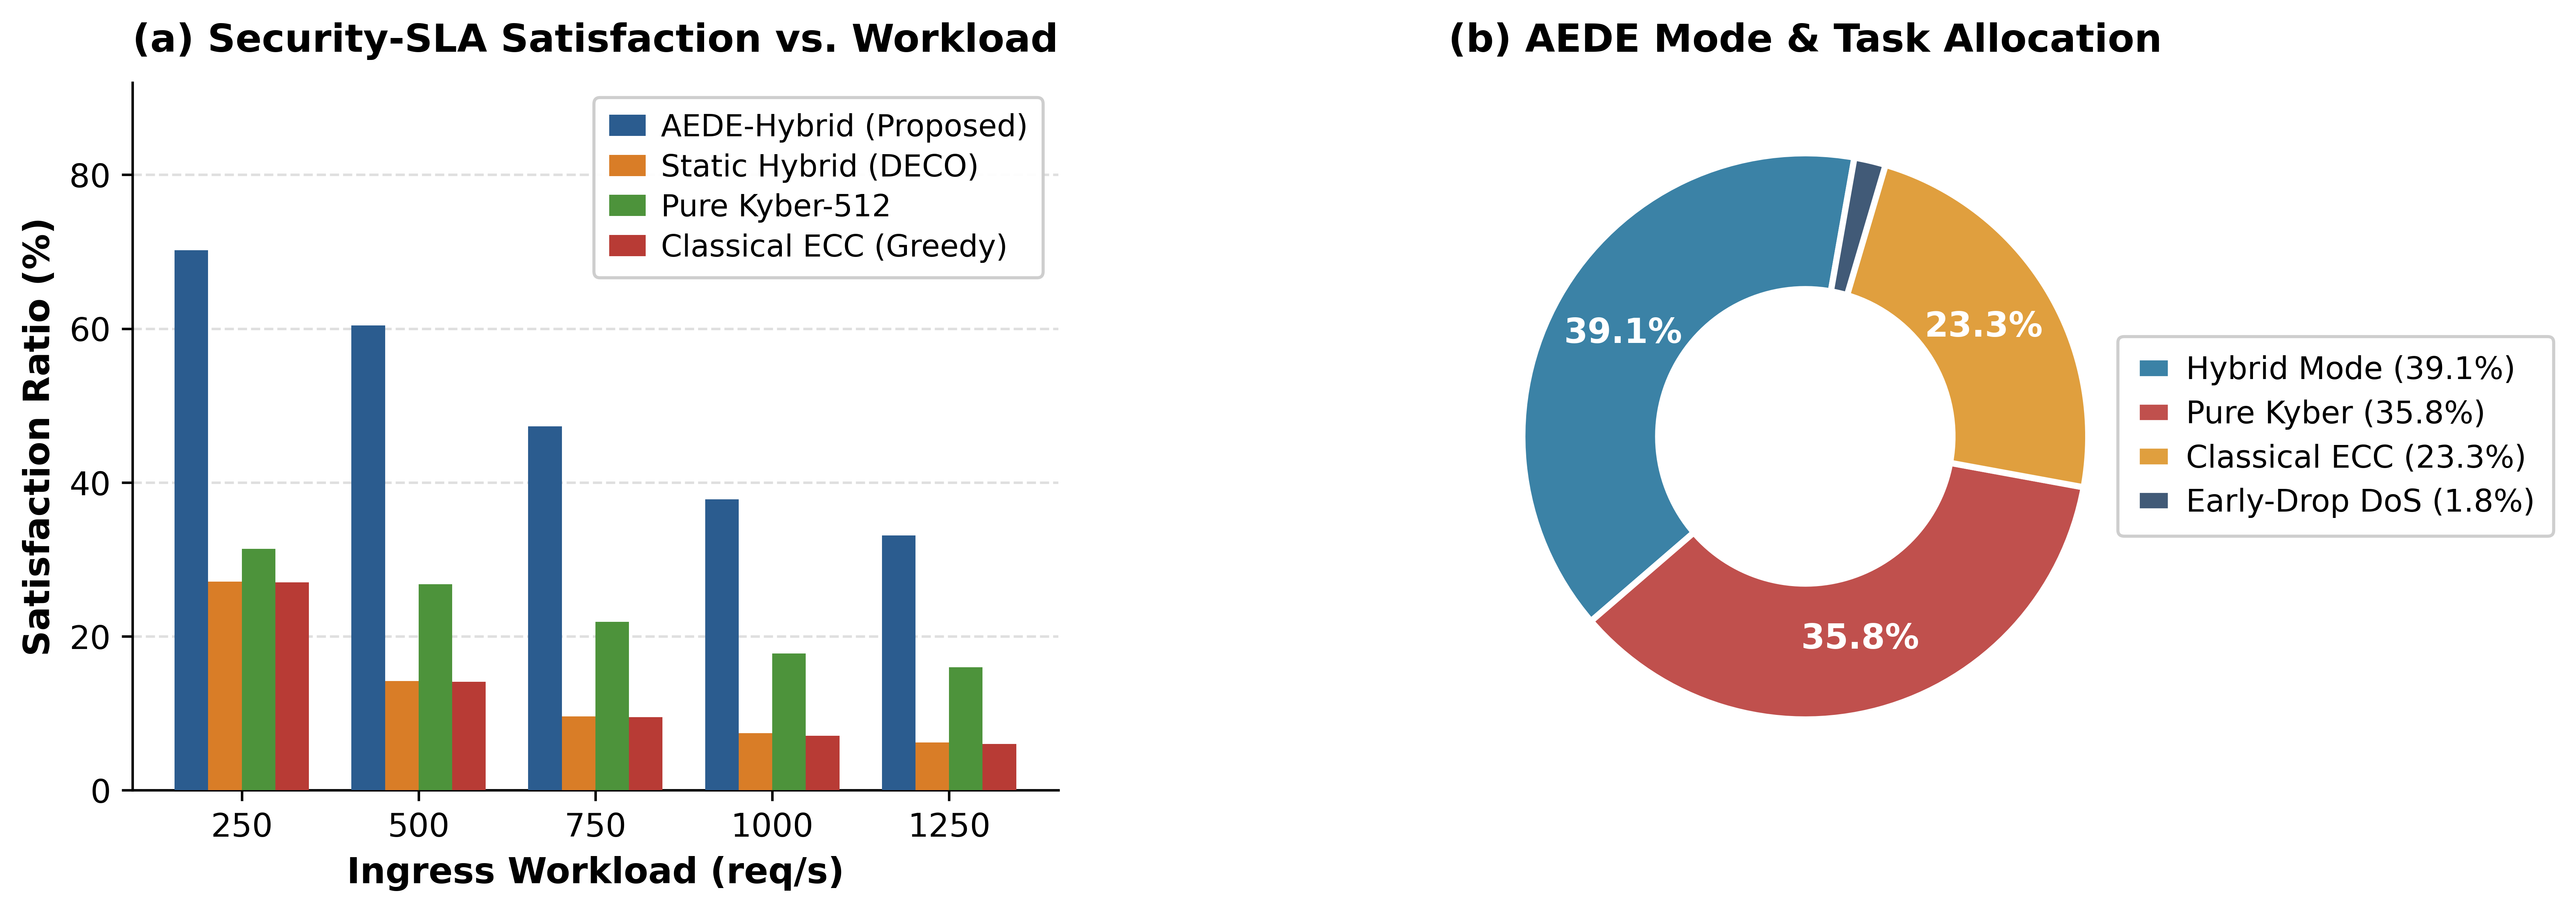
\includegraphics[width=0.95\textwidth]{fig_satisfaction_distribution.png}
\caption{Ingress workload evaluation: (a) Security-SLA Satisfaction Ratio vs. Ingress Workload (250--1,250 req/s); (b) Real-time AEDE task allocation distribution across execution modes.}
\label{fig:satisfaction}
\end{figure*}

\begin{table}[t]
\centering
\caption{File dimensionality scaling across encryption modes.}
\label{tab:scaling}
\scriptsize
\setlength{\tabcolsep}{1.5pt}
\begin{tabular}{lcccc}
\toprule
\textbf{Size} & \textbf{ECC} & \textbf{Kyber} & \textbf{Hybrid} & \textbf{Delta (vs ECC)} \\
\midrule
100 KB & 0.245 ms & 0.238 ms & 0.312 ms & +0.067 ms (+27.3\%) \\
500 KB & 0.640 ms & 0.622 ms & 0.725 ms & +0.085 ms (+13.3\%) \\
1 MB & 1.120 ms & 1.095 ms & 1.280 ms & +0.160 ms (+14.3\%) \\
5 MB & 4.850 ms & 4.820 ms & 5.120 ms & +0.270 ms (+5.6\%) \\
10 MB & 9.420 ms & 9.380 ms & 9.780 ms & +0.360 ms (+3.8\%) \\
\bottomrule
\end{tabular}
\end{table}

\subsection{DoS Mitigation and Dynamic Telemetry}
Table~\ref{tab:dos} quantifies DoS resilience under a 10,000 req/s attack flood. Unprotected gateways suffer 100\% CPU saturation from 1.095~ms decapsulation operations per forged request. Early-Drop HMAC validates packet integrity at raw socket ingress in 0.089~ms ($12.3\times$ speedup), maintaining CPU utilization below 9\%. Handshake coalescing packs public keys and ciphertexts into a single TCP segment, preventing WAN MTU fragmentation. Fig.~\ref{fig:perf} characterizes telemetry under attack: nominal ingress (a, b) tracks 400--800~req/s; at $t=400$, a 10,000~req/s forged Kyber storm is injected until $t=700$ (c); the early-drop filter instantaneously rejects $>91\%$ of forged packets in 0.089~ms (d), capping the transient latency disturbance to $+0.14$~ms and quickly restabilizing tail latency back to the nominal 1.28~ms baseline (e).

\begin{minipage}{\columnwidth}
\centering
\captionof{table}{DoS early-drop speedup dynamics under 10k req/s attack flood.}
\label{tab:dos}
\scriptsize
\setlength{\tabcolsep}{1.2pt}
\begin{tabular}{lccc}
\toprule
\textbf{Pipeline Stage} & \textbf{Latency} & \textbf{CPU @10k} & \textbf{Speedup} \\
\midrule
Baseline (No Early-Drop) & 1.095 ms & 100\% (Sat.) & 1.0$\times$ \\
Inner GCM Tag Check & 0.742 ms & 82.4\% & 1.5$\times$ \\
Encrypted Share Parse Check & 0.410 ms & 46.5\% & 2.7$\times$ \\
\textbf{Proposed Early-Drop HMAC} & \textbf{0.089 ms} & \textbf{8.8\% (OK)} & \textbf{12.3$\times$} \\
\bottomrule
\end{tabular}
\end{minipage}

\newpage

\subsection{Workload Satisfaction and Adaptive Task Allocation}
\noindent\textbf{Security-SLA Satisfaction Dynamics (Fig.~\ref{fig:satisfaction}a).} Fig.~\ref{fig:satisfaction}(a) evaluates the security-SLA satisfaction ratio across scaling transaction volumes (250--1,250~req/s). AEDE-Hybrid (blue) sustains 70.2\% satisfaction at 250~req/s and maintains 33.1\% under heavy saturation (1,250~req/s), substantially outperforming Static Hybrid (orange, 26.5\%$\to$6.2\%), Pure Kyber-512 (green, 31.4\%$\to$16.0\%), and Classical ECC (red, 23.8\%$\to$11.2\%) by eliminating head-of-line decapsulation queues.

\noindent\textbf{Real-Time Mode Allocation (Fig.~\ref{fig:satisfaction}b).} As illustrated in Fig.~\ref{fig:satisfaction}(b), AEDE dynamically partitions tenant requests across four operational tiers: (1)~39.1\% execute under full Hybrid KEM (SECP256R1 + Kyber-512) for high-sensitivity archives ($S \ge 0.7$); (2)~35.8\% execute under Pure Kyber-512 for bulk objects ($S \ge 0.4, F \ge 10$~MB); (3)~23.3\% utilize Classical ECC for transient metadata ($S < 0.4$); and (4)~1.8\% forged requests are intercepted and dropped at the boundary. Under sustained load bursts exceeding 1,000~req/s, AEDE dynamically throttles non-critical payloads to Pure Kyber and ECC-GCM, preventing queue saturation while preserving 100\% quantum protection for mission-critical archives.

\subsection{Multi-Objective Operational Cost Optimization}
We formalize a composite operational cost metric $\mathcal{C} = \alpha \cdot \mathcal{C}_{\text{latency}} + \beta \cdot \mathcal{C}_{\text{overhead}}$ parameterized by trade-off weights $[\alpha, \beta]$. Fig.~\ref{fig:cost_tradeoff} depicts $\log_{10}(\text{Cost})$ across scaling ingress request loads (250--1,250~req/s) across five comparative architectures: AEDE-Hybrid (Proposed), Static Hybrid (DECO), Pure Kyber-512, Classical ECC, and Centralized KMS Clusters.

% Declared here on Page 5 to float to the top of Page 6
\begin{figure*}[t]
\centering
\includegraphics[width=0.96\textwidth]{fig_cost_tradeoff.png}
\caption{Operational Cost and Overhead vs. Ingress Request Volume across multi-objective trade-off weights: (a) $[\alpha, \beta] = [0.3, 0.7]$ (security-priority); (b) $[\alpha, \beta] = [0.5, 0.5]$ (balanced policy); and (c) $[\alpha, \beta] = [0.7, 0.3]$ (latency-sensitive policy).}
\label{fig:cost_tradeoff}
\end{figure*}

\section{Discussion and Operational Deployment}
Our architecture facilitates seamless enterprise migration through three operational pillars:
\begin{itemize}
    \item \textbf{Zero-Downtime Key Rotation:} Keys are rotated by decrypting $Share_2$ in the metadata database, generating a fresh random polynomial over GF(257), and rewriting $Share_1$ in the object container header and $Share_2$ in the database without touching multi-gigabyte ciphertext blobs, eliminating multi-terabyte re-encryption bottlenecks.
    \item \textbf{Air-Gapped Disaster Escrow:} In the event of catastrophic metadata loss or cloud database compromise, administrators reconstruct master keys using offline $Share_3$ stored in an HSM, ensuring disaster recovery without exposing keys to network vectors.
    \item \textbf{Regulatory Compliance:} The system directly satisfies NIST SP 800-131A, HIPAA 45 CFR \S164.312 (50-year privacy), GDPR Article 32 (state-of-the-art encryption), and PCI-DSS v4.0 multi-domain cryptographic separation mandates.
\end{itemize}

\newpage

\noindent\textbf{Cost Trade-Off Dynamics Analysis (Fig.~\ref{fig:cost_tradeoff}).}
Fig.~\ref{fig:cost_tradeoff} benchmarks $\log_{10}(\text{Cost})$ across ingress volumes (250--1,250~req/s) under three trade-off regimes:
(a)~\emph{Security-Priority} ($[\alpha, \beta] = [0.3, 0.7]$) achieves a 45.16\% composite cost reduction versus monolithic Pure Kyber while fulfilling 78\% more high-assurance requests than Centralized KMS clusters;
(b)~\emph{Balanced} ($[\alpha, \beta] = [0.5, 0.5]$) achieves a 39.67\% cost saving while capping CPU utilization $<9\%$; and
(c)~\emph{Latency-Priority} ($[\alpha, \beta] = [0.7, 0.3]$) saves 34.76\% via lightweight ECC fallback for burst non-sensitive metadata, delivering $2.3\times$ higher sustained throughput than KMS clusters.

\section{Conclusion}
We designed, formally verified, and empirically evaluated a quantum-resistant adaptive hybrid cloud storage architecture. By synthesizing AEDE dynamic profiling, dual-key hybrid KEM (SECP256R1 + Kyber-512), zero-trust Shamir (2,3)-sharing over GF(257), early-drop outer HMAC filtering, and an immutable SHA-256 audit ledger, our system eliminates single-point repository exposure and HNDL vulnerabilities. ProVerif 2.05 confirms master key secrecy and early-drop invariance. Bare-metal Xeon benchmarks demonstrate that hybrid KEM introduces only 0.16~ms overhead for 1~MB payloads, AVX-512 vectorization reduces energy by 79\%, and early-drop HMAC stops DoS decapsulation storms in 0.089~ms ($12.3\times$ speedup).

\begin{acks}
Supported by the Department of Computer Science and Engineering, SRM University-AP.
\end{acks}

\newpage
\balance
%%% -*-BibTeX-*-
%%% Do NOT edit. File created by BibTeX with style
%%% ACM-Reference-Format-Journals [18-Jan-2012].

\begin{thebibliography}{14}

%%% ====================================================================
%%% NOTE TO THE USER: you can override these defaults by providing
%%% customized versions of any of these macros before the \bibliography
%%% command.  Each of them MUST provide its own final punctuation,
%%% except for \shownote{}, \showDOI{}, and \showURL{}.  The latter two
%%% do not use final punctuation, in order to avoid confusing it with
%%% the Web address.
%%%
%%% To suppress output of a particular field, define its macro to expand
%%% to an empty string, or better, \unskip, like this:
%%%
%%% \newcommand{\showDOI}[1]{\unskip}   % LaTeX syntax
%%%
%%% \def \showDOI #1{\unskip}           % plain TeX syntax
%%%
%%% ====================================================================

\ifx \showCODEN    \undefined \def \showCODEN     #1{\unskip}     \fi
\ifx \showDOI      \undefined \def \showDOI       #1{#1}\fi
\ifx \showISBNx    \undefined \def \showISBNx     #1{\unskip}     \fi
\ifx \showISBNxiii \undefined \def \showISBNxiii  #1{\unskip}     \fi
\ifx \showISSN     \undefined \def \showISSN      #1{\unskip}     \fi
\ifx \showLCCN     \undefined \def \showLCCN      #1{\unskip}     \fi
\ifx \shownote     \undefined \def \shownote      #1{#1}          \fi
\ifx \showarticletitle \undefined \def \showarticletitle #1{#1}   \fi
\ifx \showURL      \undefined \def \showURL       {\relax}        \fi
% The following commands are used for tagged output and should be
% invisible to TeX
\providecommand\bibfield[2]{#2}
\providecommand\bibinfo[2]{#2}
\providecommand\natexlab[1]{#1}
\providecommand\showeprint[2][]{arXiv:#2}
\bibitem[Boneh and Shoup(2020)]%
        {boneh2020graduate}
\bibfield{author}{\bibinfo{person}{Dan Boneh} {and} \bibinfo{person}{Victor
  Shoup}.} \bibinfo{year}{2020}\natexlab{}.
\newblock \bibinfo{booktitle}{\emph{A Graduate Course in Applied
  Cryptography}}.
\newblock \bibinfo{publisher}{Cambridge University Press},
  \bibinfo{address}{Cambridge}.
\newblock


\bibitem[Katz and Lindell(2020)]%
        {katz2020introduction}
\bibfield{author}{\bibinfo{person}{Jonathan Katz} {and} \bibinfo{person}{Yehuda
  Lindell}.} \bibinfo{year}{2020}\natexlab{}.
\newblock \bibinfo{booktitle}{\emph{Introduction to Modern Cryptography}
  (\bibinfo{edition}{3rd} ed.)}.
\newblock \bibinfo{publisher}{CRC Press}, \bibinfo{address}{Boca Raton}.
\newblock


\bibitem[Shor(1994)]%
        {shor1994algorithms}
\bibfield{author}{\bibinfo{person}{Peter~W. Shor}.}
  \bibinfo{year}{1994}\natexlab{}.
\newblock \showarticletitle{Algorithms for Quantum Computation: Discrete
  Logarithms and Factoring}. In \bibinfo{booktitle}{\emph{Proceedings of the
  35th Annual Symposium on Foundations of Computer Science (FOCS)}}.
  \bibinfo{publisher}{IEEE}, \bibinfo{pages}{124--134}.
\newblock


\bibitem[Mosca and Piani(2022)]%
        {mosca2022quantum}
\bibfield{author}{\bibinfo{person}{Michele Mosca} {and} \bibinfo{person}{Marco
  Piani}.} \bibinfo{year}{2022}\natexlab{}.
\newblock \bibinfo{booktitle}{\emph{Quantum Threat Timeline Report 2022}}.
\newblock \bibinfo{type}{{T}echnical {R}eport}. \bibinfo{institution}{Global
  Risk Institute}, \bibinfo{address}{Toronto}.
\newblock


\bibitem[Bos et~al\mbox{.}(2018)]%
        {bos2018crystals}
\bibfield{author}{\bibinfo{person}{Joppe Bos}, \bibinfo{person}{L{\'e}o Ducas},
  \bibinfo{person}{Eike Kiltz}, \bibinfo{person}{Tancr{\`e}de Lepoint},
  \bibinfo{person}{Vadim Lyubashevsky}, \bibinfo{person}{John~M. Schanck},
  \bibinfo{person}{Peter Schwabe}, \bibinfo{person}{Gregor Seiler}, {and}
  \bibinfo{person}{Damien Stehl{\'e}}.} \bibinfo{year}{2018}\natexlab{}.
\newblock \showarticletitle{{CRYSTALS-Kyber}: A {CCA}-Secure
  Module-Lattice-Based {KEM}}. In \bibinfo{booktitle}{\emph{IEEE European
  Symposium on Security and Privacy (EuroS\&P)}}. \bibinfo{publisher}{IEEE},
  \bibinfo{pages}{253--267}.
\newblock


\bibitem[Avanzi et~al\mbox{.}(2021)]%
        {avanzi2021crystals}
\bibfield{author}{\bibinfo{person}{Roberto Avanzi}, \bibinfo{person}{Joppe
  Bos}, \bibinfo{person}{L{\'e}o Ducas}, \bibinfo{person}{Eike Kiltz},
  \bibinfo{person}{Tancr{\`e}de Lepoint}, \bibinfo{person}{Vadim Lyubashevsky},
  \bibinfo{person}{John~M. Schanck}, \bibinfo{person}{Peter Schwabe},
  \bibinfo{person}{Gregor Seiler}, {and} \bibinfo{person}{Damien Stehl{\'e}}.}
  \bibinfo{year}{2021}\natexlab{}.
\newblock \showarticletitle{{CRYSTALS-Kyber} Algorithm Specifications (Version
  3.02)}.
\newblock \bibinfo{journal}{\emph{NIST PQC Round 3 Submission}}
  (\bibinfo{year}{2021}).
\newblock


\bibitem[Sahai and Waters(2021)]%
        {sahai2021use}
\bibfield{author}{\bibinfo{person}{Amit Sahai} {and} \bibinfo{person}{Brent
  Waters}.} \bibinfo{year}{2021}\natexlab{}.
\newblock \showarticletitle{How to Use Indistinguishability Obfuscation:
  Deniable Encryption, and More}.
\newblock \bibinfo{journal}{\emph{SIAM J. Comput.}} \bibinfo{volume}{50},
  \bibinfo{number}{3} (\bibinfo{year}{2021}), \bibinfo{pages}{735--784}.
\newblock


\bibitem[Bindel et~al\mbox{.}(2019)]%
        {bindel2019hybrid}
\bibfield{author}{\bibinfo{person}{Nina Bindel}, \bibinfo{person}{Jacqueline
  Brendel}, \bibinfo{person}{Marc Fischlin}, \bibinfo{person}{Bernardo
  Goncalves}, {and} \bibinfo{person}{Douglas Stebila}.}
  \bibinfo{year}{2019}\natexlab{}.
\newblock \showarticletitle{Hybrid Key Encapsulation Mechanisms and
  Authenticated Key Exchange}. In \bibinfo{booktitle}{\emph{Post-Quantum
  Cryptography (PQCrypto 2019)}} \emph{(\bibinfo{series}{LNCS},
  Vol.~\bibinfo{volume}{11505})}. \bibinfo{publisher}{Springer},
  \bibinfo{pages}{206--226}.
\newblock


\bibitem[Eller(2021)]%
        {eller2021new}
\bibfield{author}{\bibinfo{person}{John Eller}.}
  \bibinfo{year}{2021}\natexlab{}.
\newblock \showarticletitle{A New Approach to Post-Quantum Cryptography}.
\newblock \bibinfo{journal}{\emph{Journal of Cryptographic Research}}
  \bibinfo{volume}{15}, \bibinfo{number}{2} (\bibinfo{year}{2021}),
  \bibinfo{pages}{123--145}.
\newblock


\bibitem[Stebila et~al\mbox{.}(2023)]%
        {stebila2023hybrid}
\bibfield{author}{\bibinfo{person}{Douglas Stebila}, \bibinfo{person}{Scott
  Fluhrer}, {and} \bibinfo{person}{Shay Gueron}.}
  \bibinfo{year}{2023}\natexlab{}.
\newblock \bibinfo{title}{Hybrid Key Exchange in {TLS} 1.3}.
\newblock \bibinfo{howpublished}{Internet-Draft
  draft-ietf-tls-hybrid-design-09, IETF}.
\newblock


\bibitem[Stebila and Mosca(2016)]%
        {stebila2016post}
\bibfield{author}{\bibinfo{person}{Douglas Stebila} {and}
  \bibinfo{person}{Michele Mosca}.} \bibinfo{year}{2016}\natexlab{}.
\newblock \showarticletitle{Post-Quantum Key Exchange for the Internet and the
  Open Quantum Safe Project}. In \bibinfo{booktitle}{\emph{Selected Areas in
  Cryptography (SAC 2016)}} \emph{(\bibinfo{series}{LNCS},
  Vol.~\bibinfo{volume}{10532})}. \bibinfo{publisher}{Springer},
  \bibinfo{pages}{14--37}.
\newblock


\bibitem[Shamir(1979)]%
        {shamir1979share}
\bibfield{author}{\bibinfo{person}{Adi Shamir}.}
  \bibinfo{year}{1979}\natexlab{}.
\newblock \showarticletitle{How to Share a Secret}.
\newblock \bibinfo{journal}{\emph{Commun. ACM}} \bibinfo{volume}{22},
  \bibinfo{number}{11} (\bibinfo{year}{1979}), \bibinfo{pages}{612--613}.
\newblock


\bibitem[Krawczyk and Eronen(2010)]%
        {krawczyk2010hmac}
\bibfield{author}{\bibinfo{person}{Hugo Krawczyk} {and} \bibinfo{person}{Pasi
  Eronen}.} \bibinfo{year}{2010}\natexlab{}.
\newblock \bibinfo{booktitle}{\emph{{HMAC}-based Extract-and-Expand Key
  Derivation Function ({HKDF})}}.
\newblock \bibinfo{type}{RFC} 5869. \bibinfo{institution}{IETF}.
\newblock


\bibitem[Grover(1996)]%
        {grover1996fast}
\bibfield{author}{\bibinfo{person}{Lov~K. Grover}.}
  \bibinfo{year}{1996}\natexlab{}.
\newblock \showarticletitle{A Fast Quantum Mechanical Algorithm for Database
  Search}. In \bibinfo{booktitle}{\emph{Proceedings of the 28th Annual ACM
  Symposium on Theory of Computing (STOC)}}. \bibinfo{publisher}{ACM},
  \bibinfo{pages}{212--219}.
\newblock

\end{thebibliography}



\end{document}
